\documentclass[12pt, letterpaper]{article}
\usepackage[utf8]{inputenc}
\usepackage{graphicx}
\usepackage{hyperref}
\usepackage{fancyvrb}
\usepackage{array}
\usepackage{biblatex}
\usepackage{float}
\usepackage{subcaption}

\bibliography{rapport}

\title{Off-Line Handwritten Character Recognition System Using Support Vector Machine}
\author{Komlan Jean-Marie DANTODJI
\\
    \multicolumn{1}{
        p{.7\textwidth}}{\centering\emph{Université Paris Vincennes St-Denis\\
  M1 Big Data\\}
  }
}
\date{\today}
\begin{document}


\begin{titlepage}
    \maketitle
\end{titlepage}

\tableofcontents

\newpage
\section{Introduction à la méthode du SVM : Support Vector Machine}
\par Proposé par Boser, Guyon, et Vapnik en 1992, SVM est une technique de classification linéaire et non linéaire.\\
\subsection{Linéarité séparable}
\par SVM est un modèle d’apprentissage supervisé basé sur la détermination d’un hyperplan qui sépare les données d’une classe des autres classes.
\begin{figure}[H]
    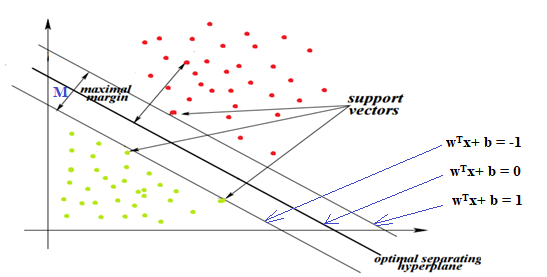
\includegraphics[width=\linewidth]{images/svm_separate.png}
    \caption{Détermination de l’hyperplan}
    \label{fig:L1}
\end{figure}
\par L’objectif du SVM est de déterminer l’hyperplan qui sépare une classe des autres avec une marge maximale M.  \\
Soit $x_0$ et $x_1$ deux vecteurs supports aux deux extrémités et
Soit l' hyperplant $$(P): w^Tx+b=0$$

$$M = d(x_{0},P)+d(x_{1},P) = \frac{\mid{w^{T}x_{0}+b}\mid}{\sqrt{w^{T}w} } + \frac{\mid{w^{T}x_{1}+b}\mid}{\sqrt{w^{T}w} } $$

$$ = \frac{\mid{1}\mid}{\sqrt{w^{T}w} } + \frac{\mid{-1}\mid}{\sqrt{w^{T}w}} = \frac{2}{\sqrt{w^{T}w} }$$  
\par Maximiser M revient à minimiser $$\frac{\sqrt{w^{T}w}}{2} = \frac{\|w\|}{2}$$

\subsection{Linéarité inséparable}
\begin{figure}[H]
    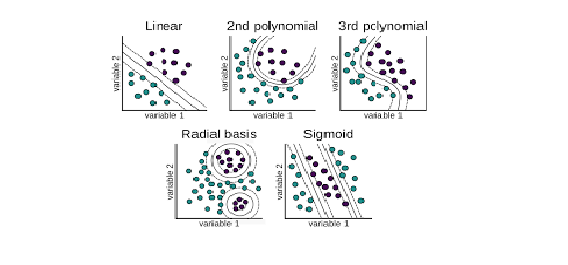
\includegraphics[width=\linewidth]{images/svm_non_linear.png}
    \caption{Inséparabilité linéaire : https://www.r-bloggers.com/2019/10/support-vector-machines-with-the-mlr-package/}
    \label{fig:L1}
\end{figure}
\par Dans ces cas d’inséparabilité linéaire on peut utiliser des fonctions de kernel notamment :\\
Kernel linéaire: $$  K(X_{i},X_{j})=x_i^T x_j$$\\
Kernel Polynomial:  $$K(X_i,X_j ) = (\gamma x_i^T x_j+r)^d$$\\
Kernel Radial: $$K(X_i,X_j ) = \mathrm{e}^{\gamma(x_i-x_j )^2}$$\\
Kernel Sigmoid: $$K(X_i,X_j )= \tanh{(\gamma x_i^T x_j+r)}$$
\section{Etapes de prétraitement:} 
\par Pour implémenter ce model on s’est servi des données de la base de sonnée de CENPARMI, CEDAR et MNIST). Une première étape est le prétraitement de l’image contenant le texte manuscrit permettant une bonne extraction des caractéristiques. \\
\par Les différentes étapes de prétraitement :
\begin{figure}[H]
    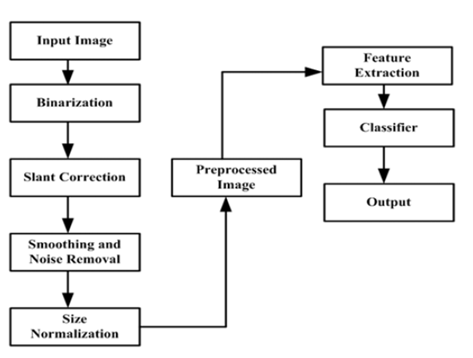
\includegraphics[width=12cm,height=10cm]{images/pretraitement.png}
    \caption{Etapes de prétraitement de l’image : http://www.sciencepublishinggroup.com/j/ajnna}
    \label{fig:L1}
\end{figure}
\begin{itemize}
		\item Binarization :\\
		L’image est convertie en niveau de gris pour éviter les problèmes causés par les bruits nuisible à l’extraction des caractéristiques
		\item Slant Correction :\\
		Correction de l’inclinaison, Procéder à un repositionnement de l’image si elle n’est pas droite.
		\item Smoothing and Noise Removal : \\
		Polir et éliminer les bruits
		\item Size Normalization : \\
		Normaliser la taille des caractères pour avoir la même dimension.
\end{itemize}
\section{Extraction des caractéristiques}
\par Pour chaque caractère récupéré on a besoin des caractéristiques qui peuvent la représenter. Pour cela on distingue plusieurs méthodes d’extraction de caractéristique dont la méthode de Diagonal distance : 
\begin{figure}[H]
    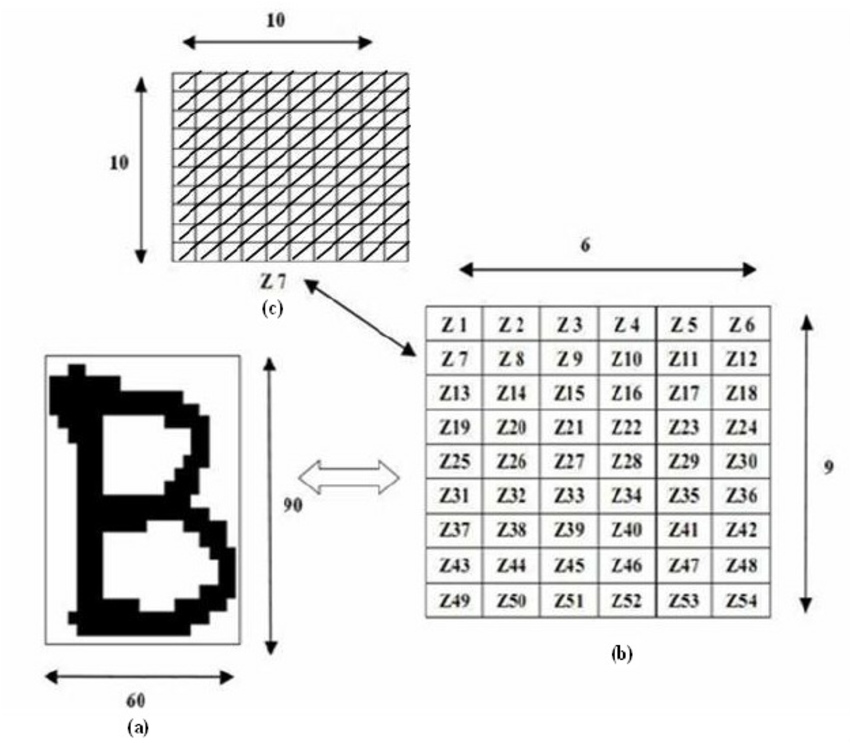
\includegraphics[width=12cm,height=8cm]{images/diagonal_methode.png}
    \caption{Méthode d'extraction diagonale: https://www.researchgate.net/figure/Procedure-for-extracting-feature-from-the-characters}
    \label{fig:L1}
\end{figure}


\section{Model de SVM }
\par Pour avoir plus une meilleure classification on utilise le Kernel polynomial pour avoir une meilleure séparation des classes de chaque caractère.\\
\par Les différents étapes de SVM :\\
\begin{figure}[H]
    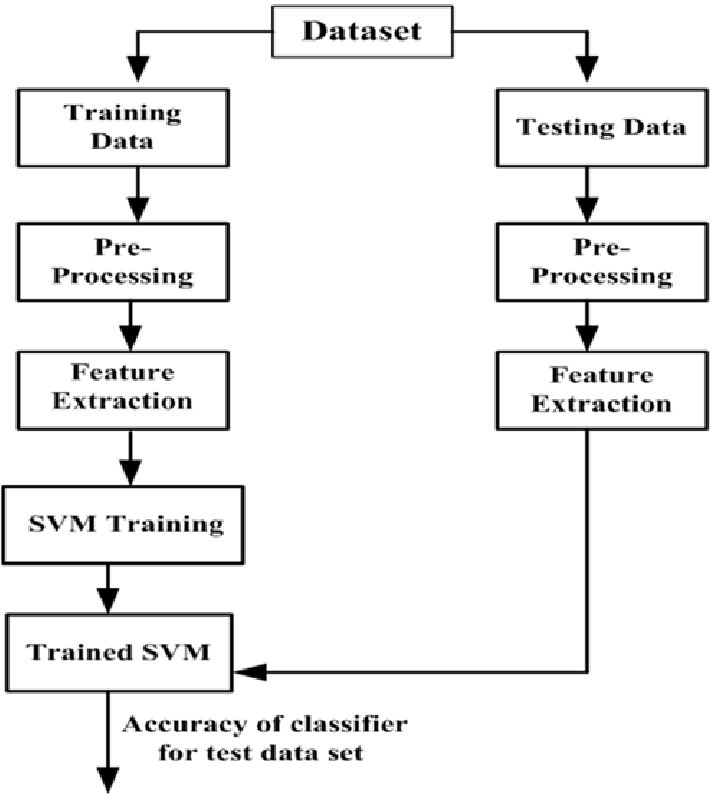
\includegraphics[width=12cm,height=10cm]{images/svm_methode.png}
    \caption{Etapes de SVM: https://www.researchgate.net/figure/Different-stages-of-SVM-classification}
    \label{fig:L1}
\end{figure}


\newpage
\section{Synthèse et Conclusion}
\par La précision de la méthode de SVM en l’appliquant à la base de donnée CED AR CDROM est définie dans le tableau suivant : 
\begin{figure}[H]
    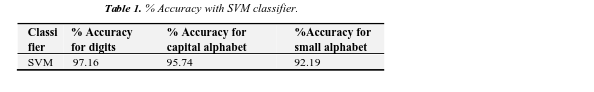
\includegraphics[width=25cm,height=5cm]{images/accuracy.png}
    \caption{https://www.researchgate.net/publication/323112207Off-Line Handwritten Character Recognition System Using Support Vector Machine}
    \label{fig:L1}
\end{figure}


\section{Reférences}
\par [1] Gauri Katiyar, Ankita Katiyar, Shabana Mehfuz ont écrit la revue Off-Line Handwritten Character Recognition System Using Support Vector Machine publié dans le journal  American Journal of Neural Networks and Applications le 13 décembre 2017.


\newpage
\printbibliography
\end{document}
